\chapter{Results and Discussion}\label{Sec:Results}

\section{Experimental Uncertainty of Shock Tube IDT Data}
\subsection{shen vs davidson}
\begin{figure}[htbp]
	\centering
	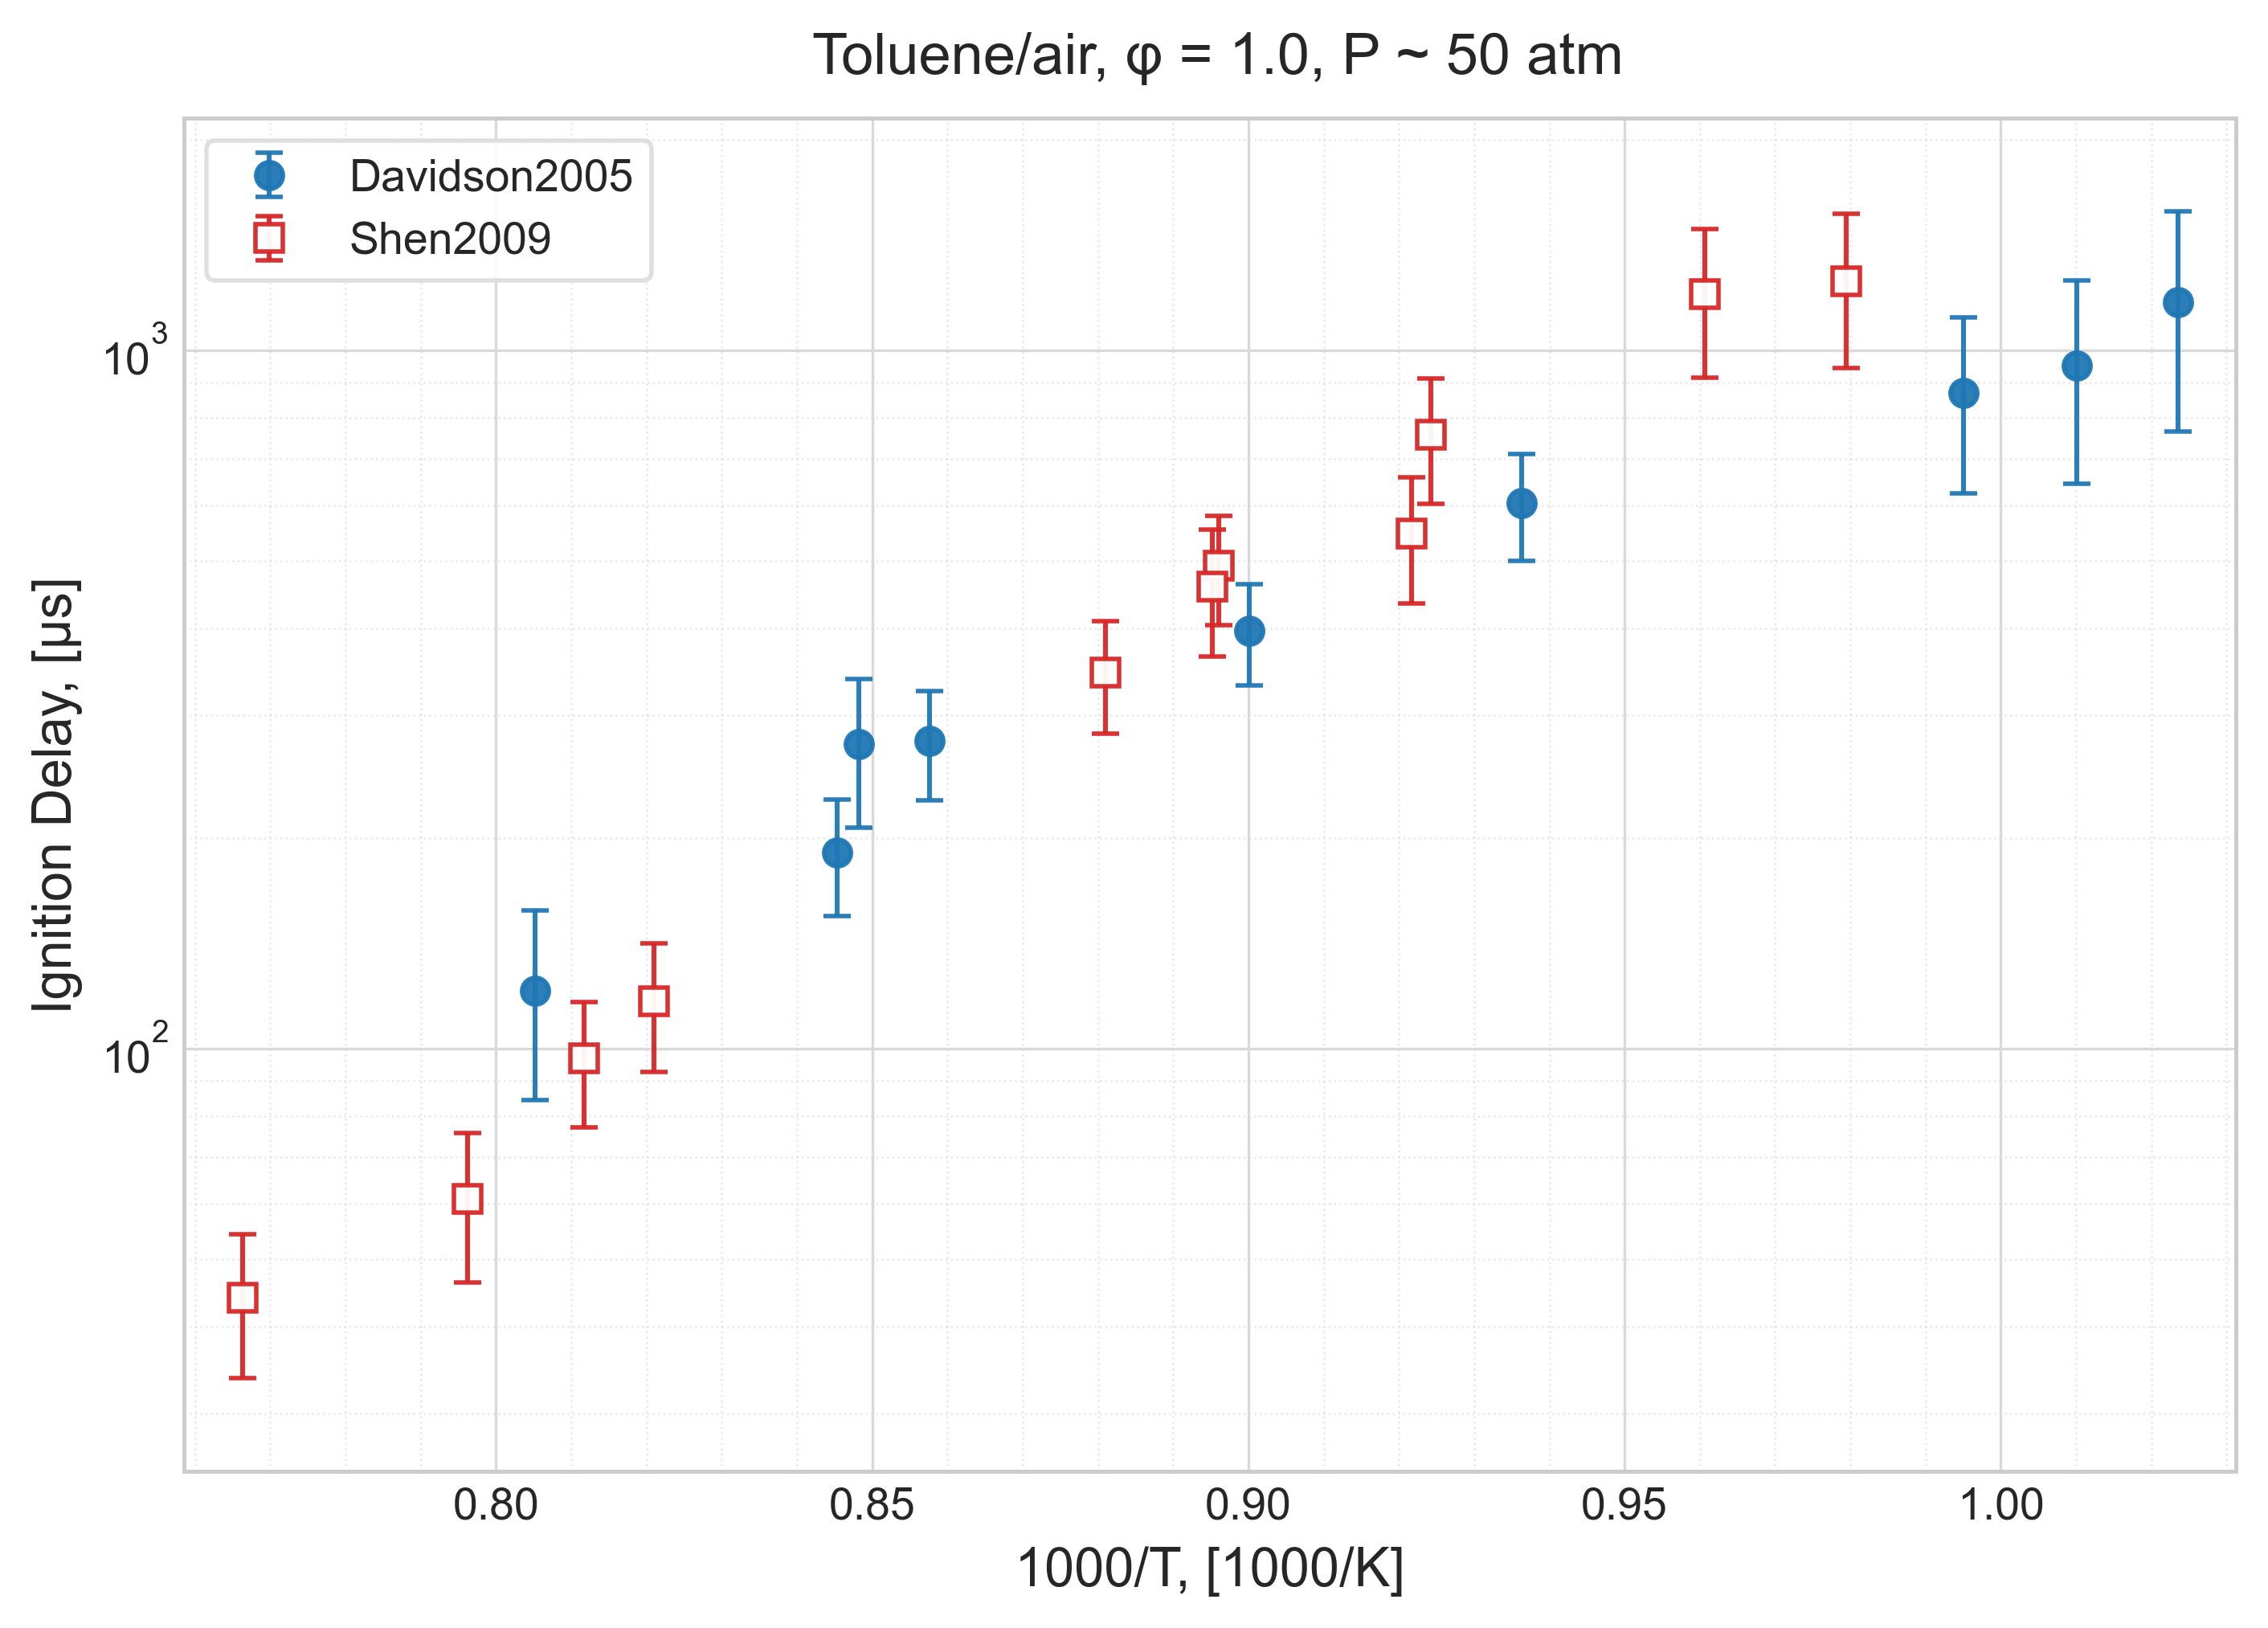
\includegraphics[width=0.8\textwidth]{Figures/davidson_2005_shen_2009_ignition_delay.png}
	\caption{Comparison of calculated IDT uncertainties for a stoichiometric toluene/air mixture. IDT measurements are from two different facilities \cite{shen_shock_2009}\cite{davidson_shock_2005} over similar temperature range. P$\sim$50 atm.}
	\label{fig:davidson_shen}
\end{figure}
\subsection{Syngas}

\begin{figure}[htbp]
	\centering
	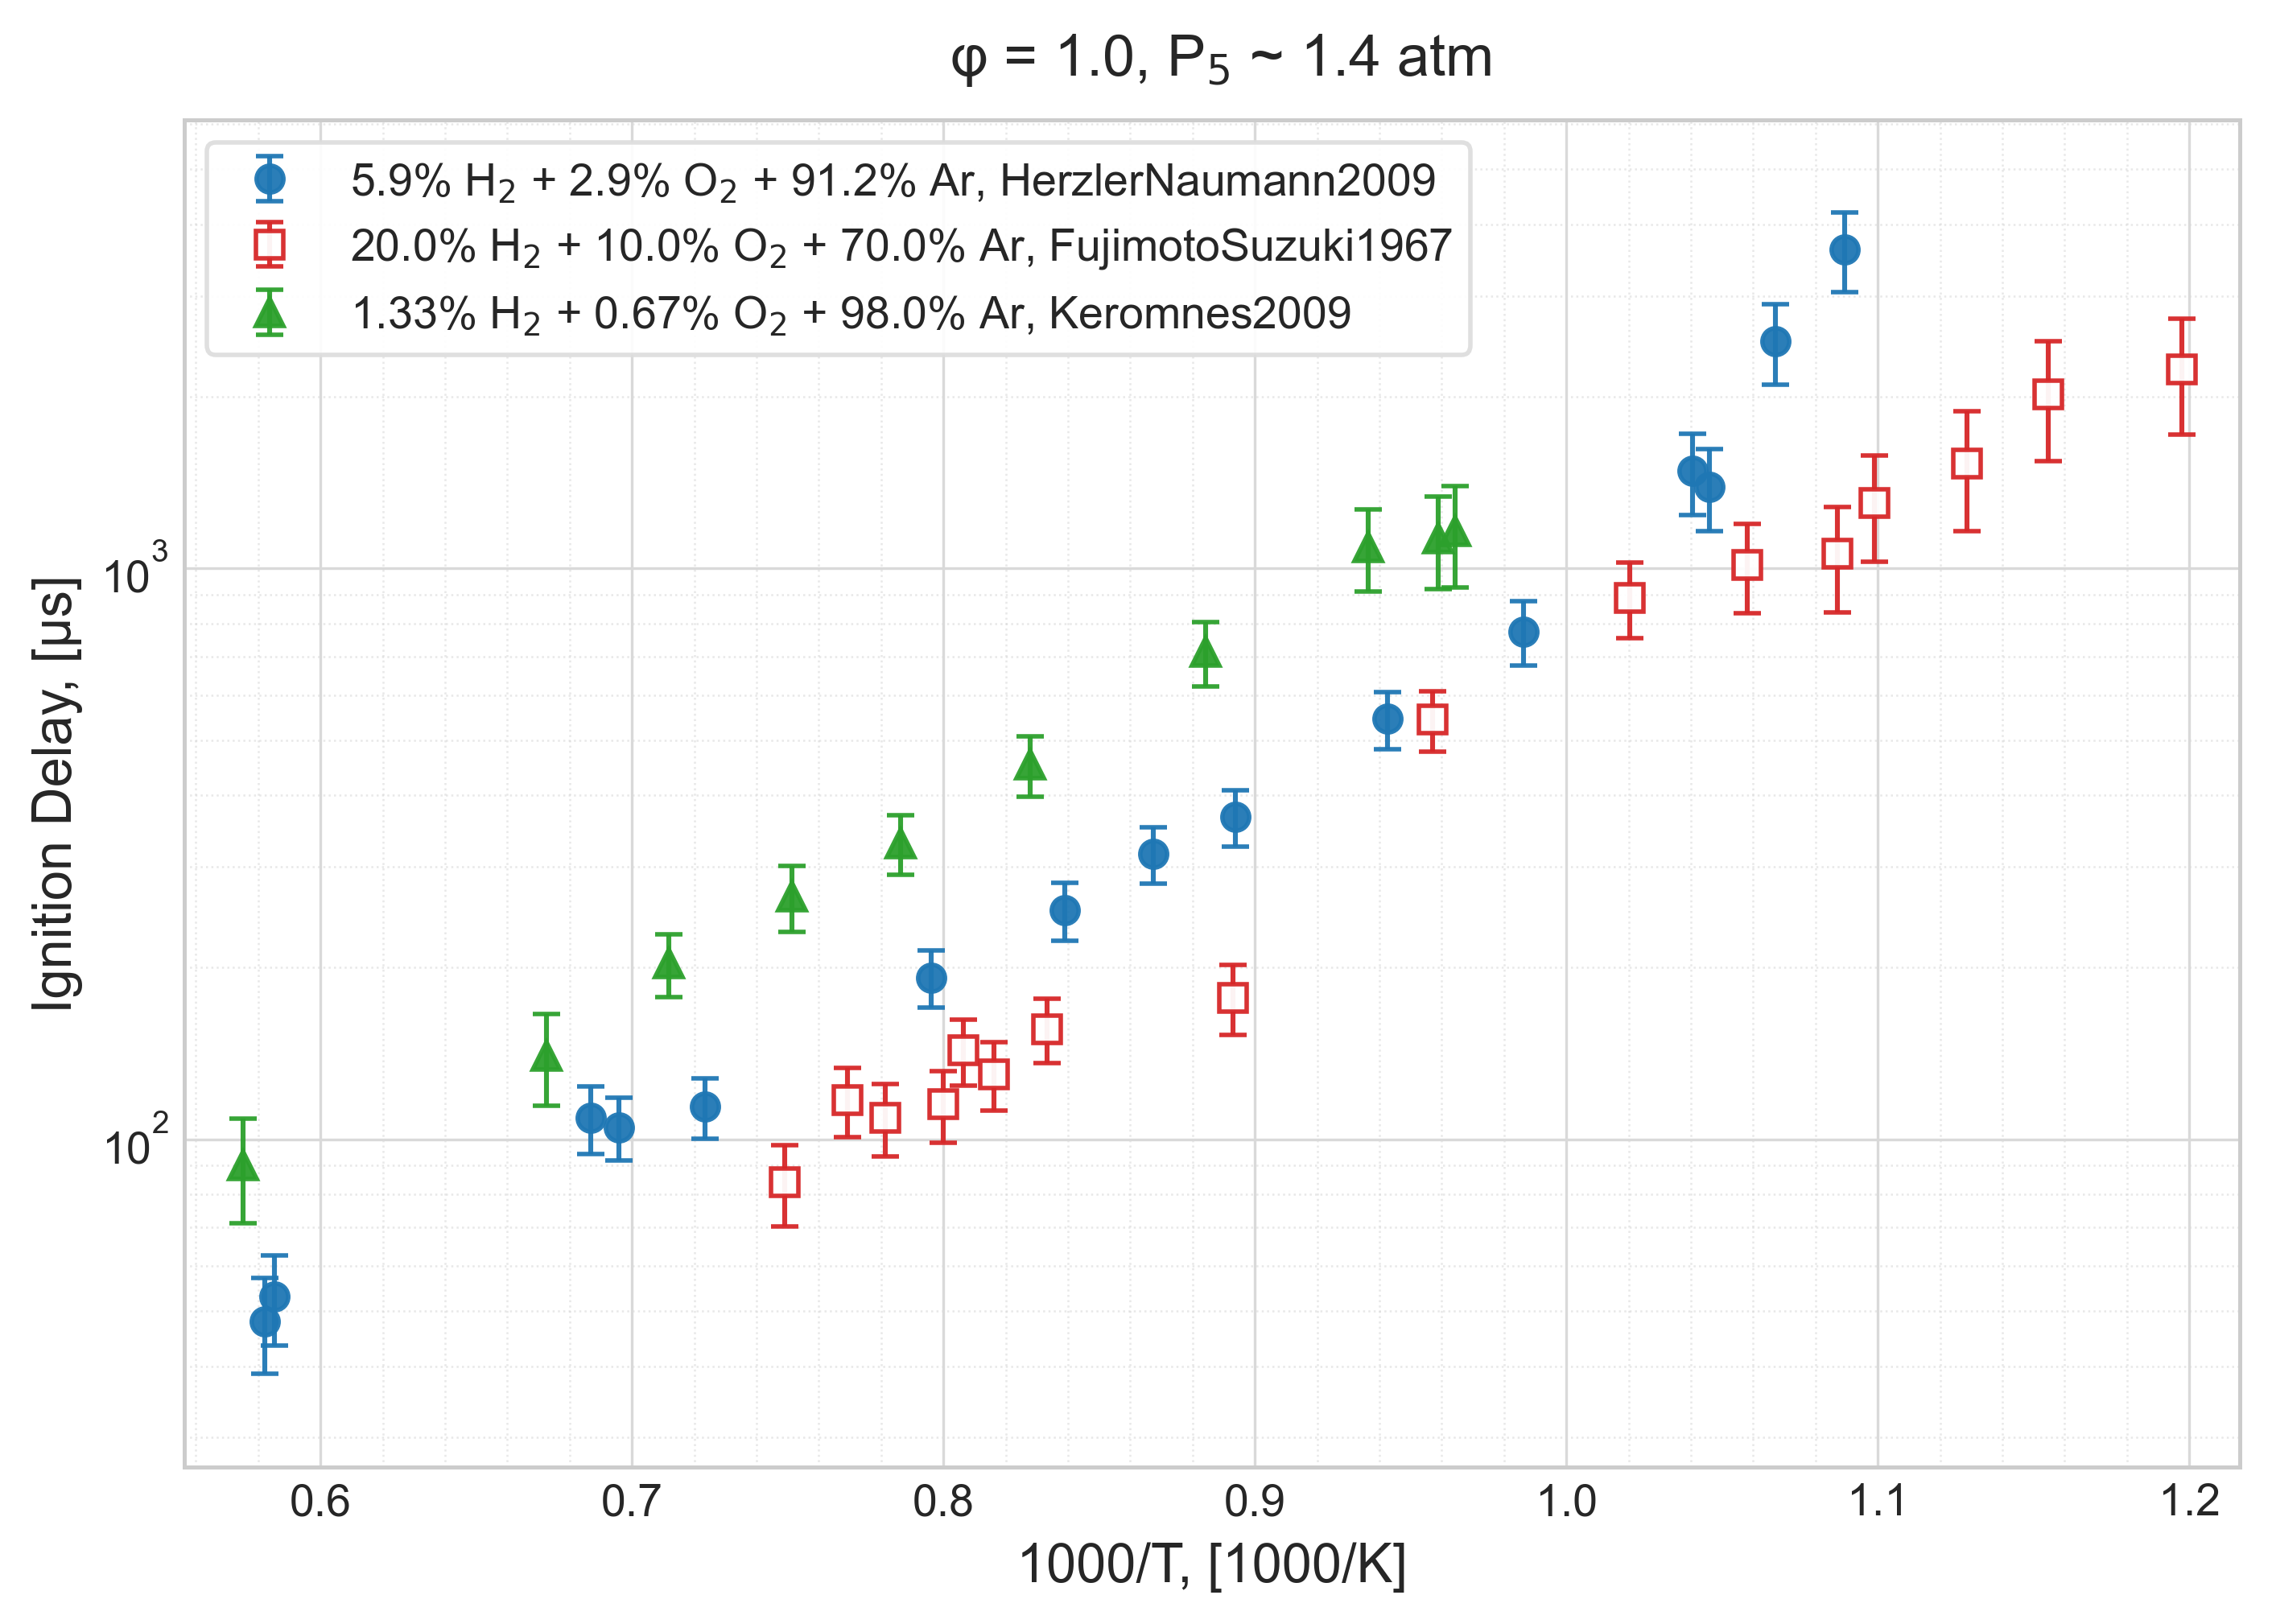
\includegraphics[width=0.8\textwidth]{Figures/g00000012_x10000006_x10000039_ignition_delay.png}
	\caption{Comparison of calculated IDT uncertainties for $H_2/O_2/Ar$ mixtures. IDT measurements are from sources \cite{herzler_shock-tube_2009} \cite{chemical_kinetics_laboratory_fujimoto_2017} \cite{keromnes_experimental_2013}.$\phi = 1.0, P\sim 1.4 atm$.}
	\label{fig:hydrogen_compare}
\end{figure}

\begin{figure}[htbp]
	\centering
	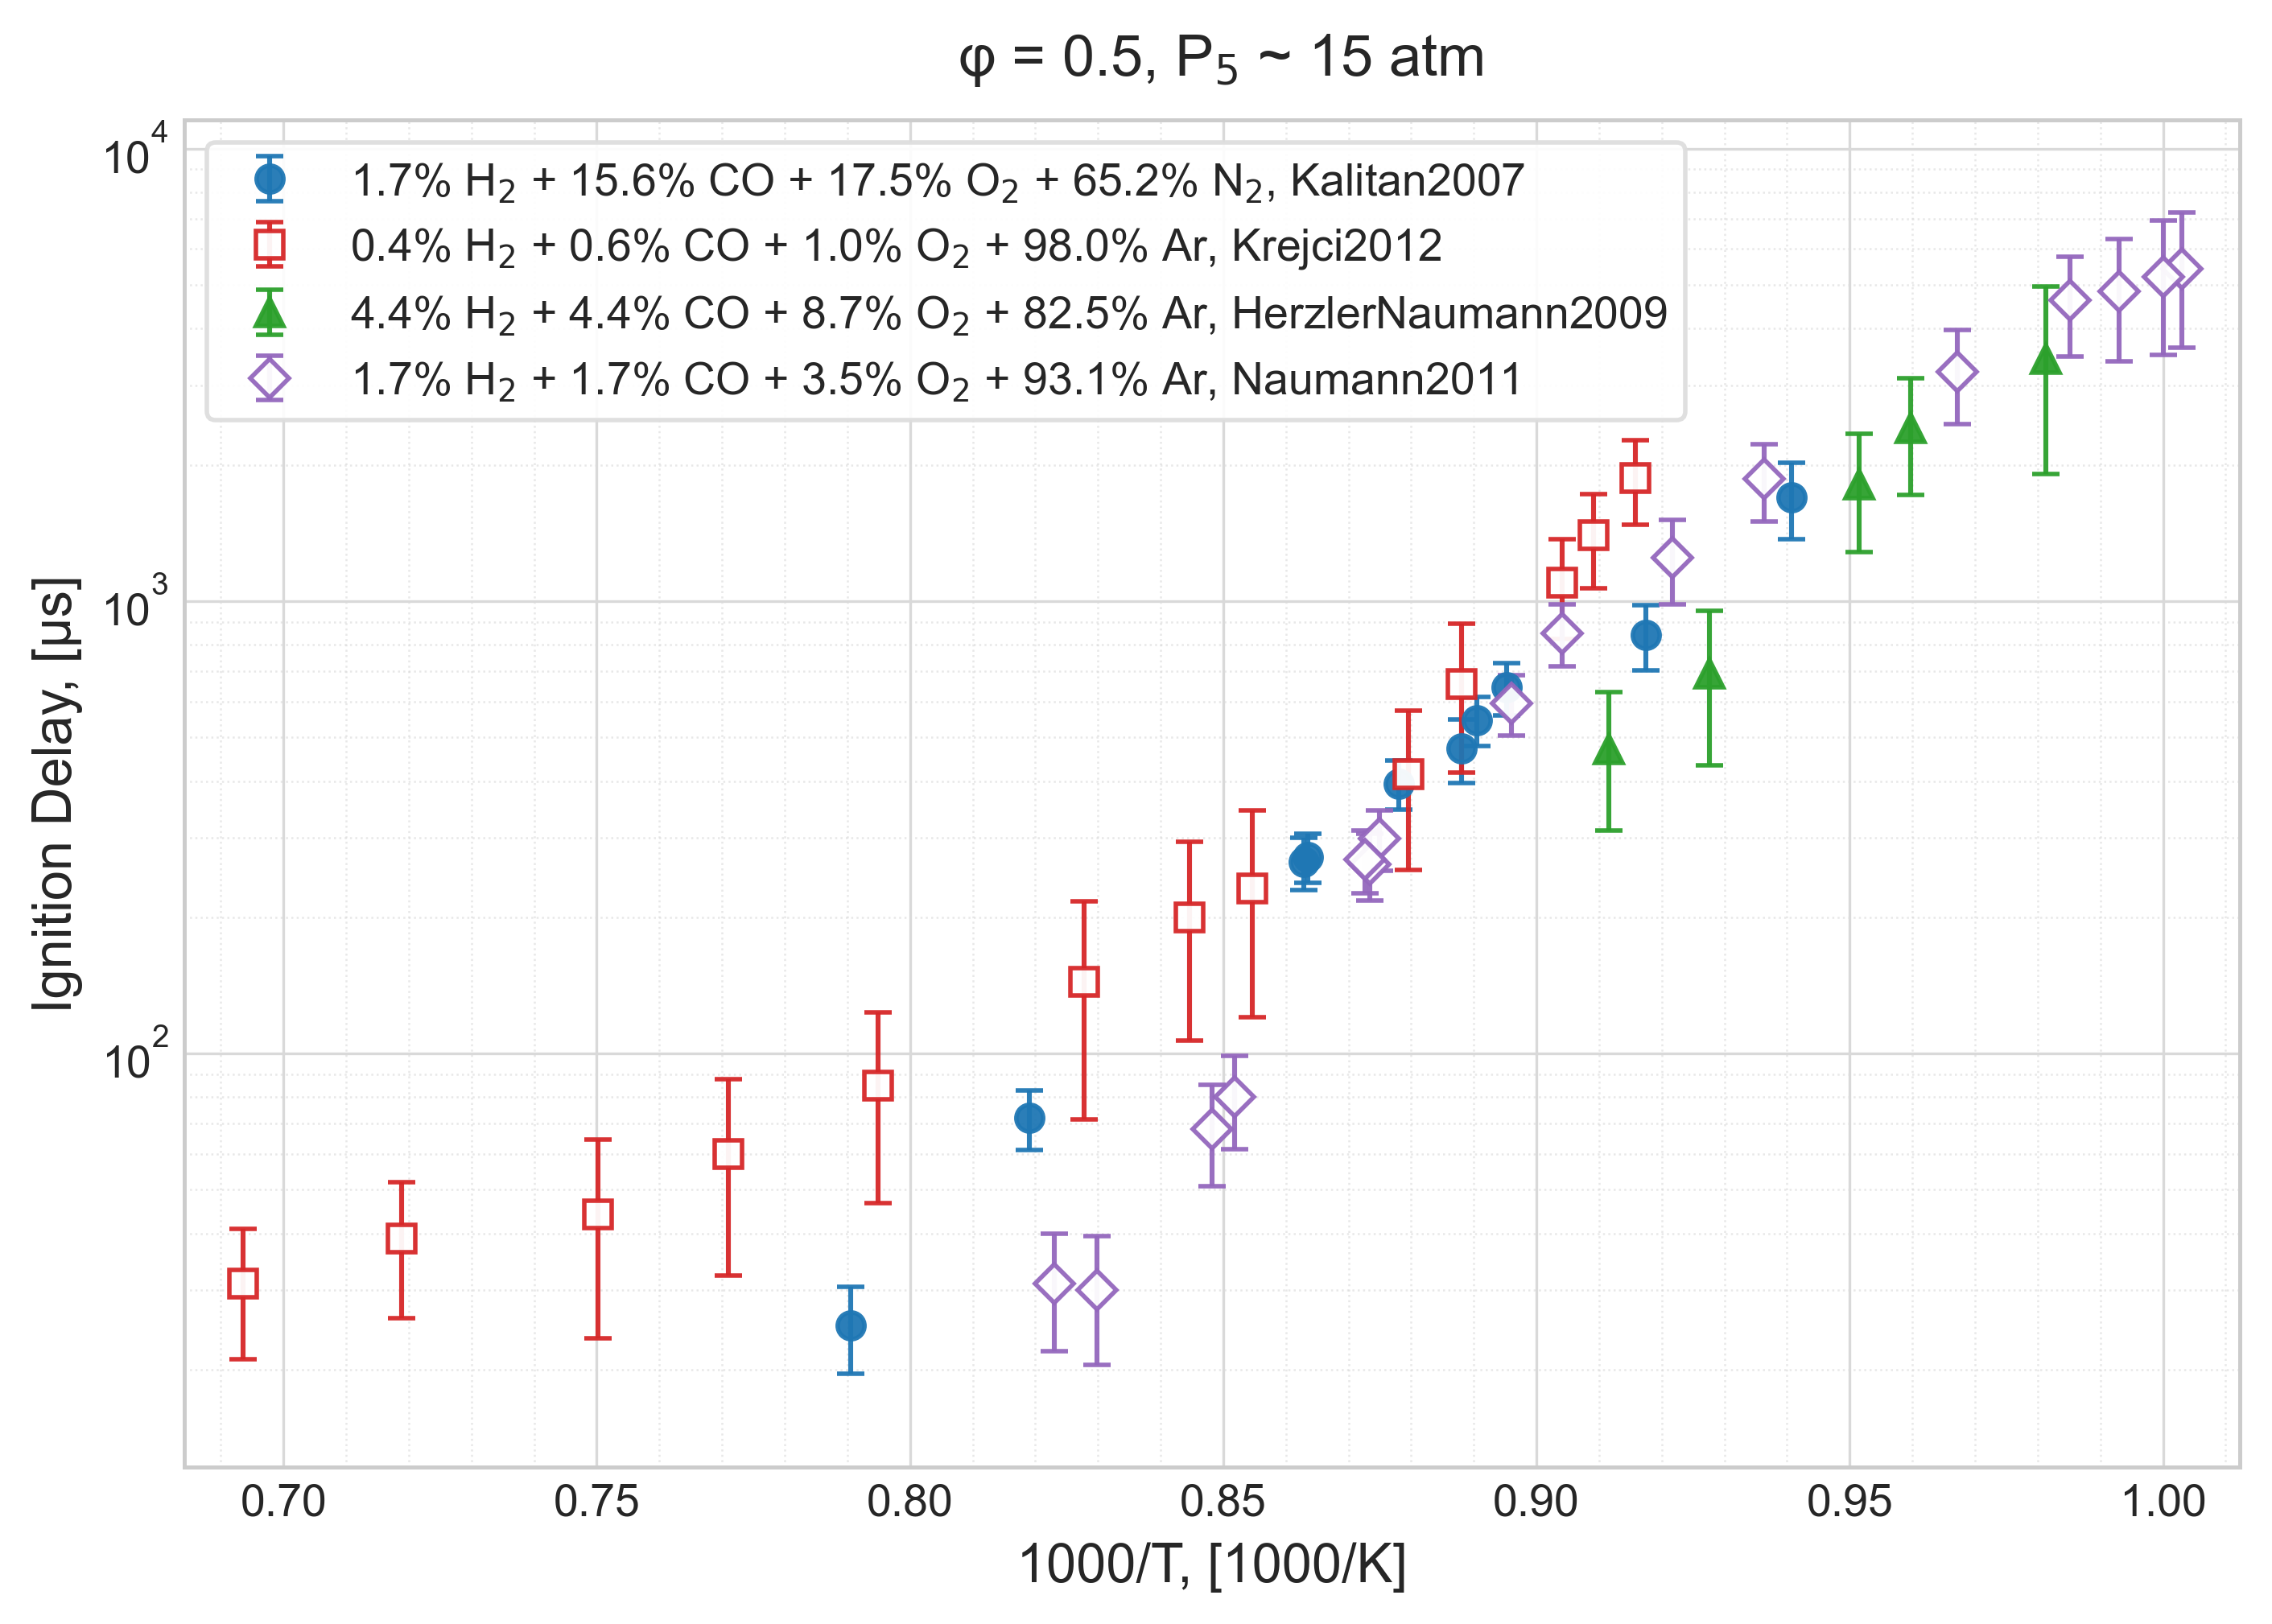
\includegraphics[width=0.8\textwidth]{Figures/x10001041_x10001066_x10001056_x10001024_x_ignition_delay.png}
	\caption{Comparison of calculated IDT uncertainties for diluted syngas/oxidizer mixtures. IDT measurements are from sources \cite{kalitan_ignition_2007} \cite{krejci_laminar_2012} \cite{herzler_shock-tube_2009} \cite{chemical_kinetics_laboratory_c_2017}$\phi = 0.5, P\sim 15 atm$.}
	\label{fig:syngas_compare}
\end{figure}

for most reported sources shock tube setup specific information is not available in an easily accessable database. They are available in the original papers,however to extract them would require manual entry, for programmatic processing with language model. This is necessary for an accurate estimation of experimental shock tube IDT uncertainties. 


\section{Cantera Shock Tube IDT Simulations}
\begin{figure}[htbp]
	\centering
	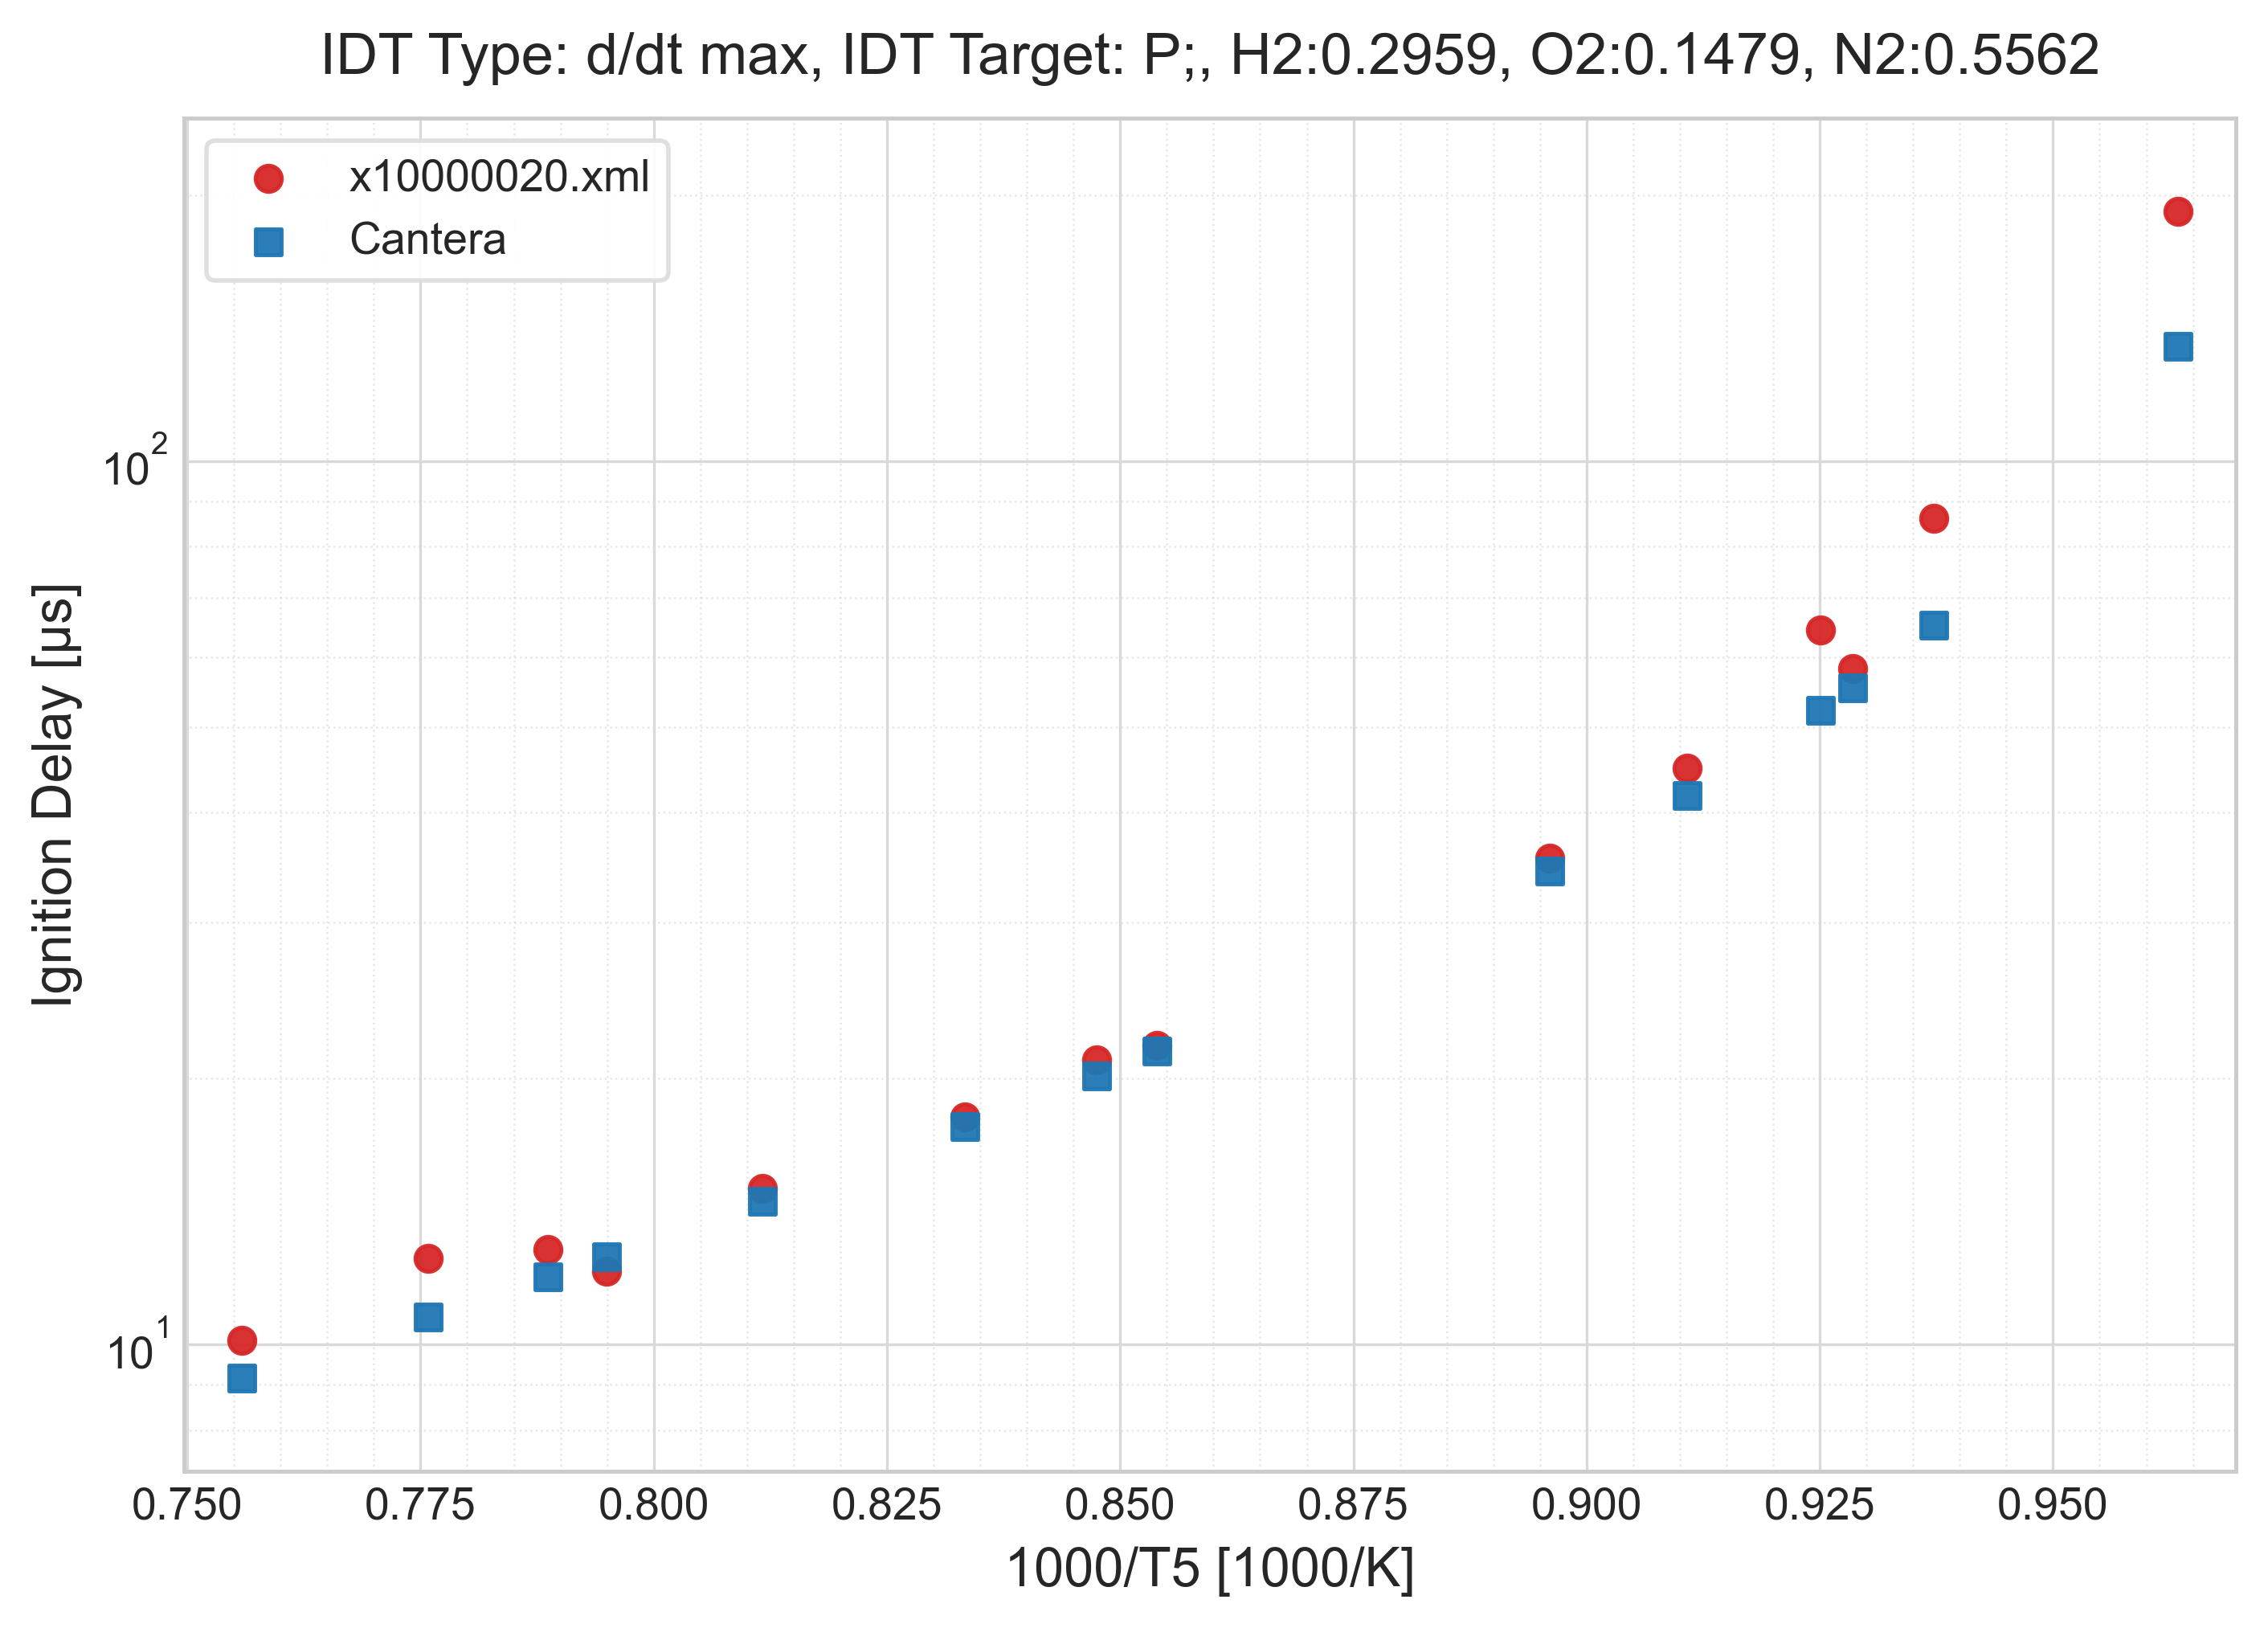
\includegraphics[width=0.8\textwidth]{Figures/IDT_plot_x10000020.png}
	\caption{Comparison of Cantera IDT simulation with experimental measurement \cite{good_cantera} IDT Type: dP/dt max.}
	\label{fig:good_cantera}
\end{figure}
\begin{figure}[htbp]
	\centering
	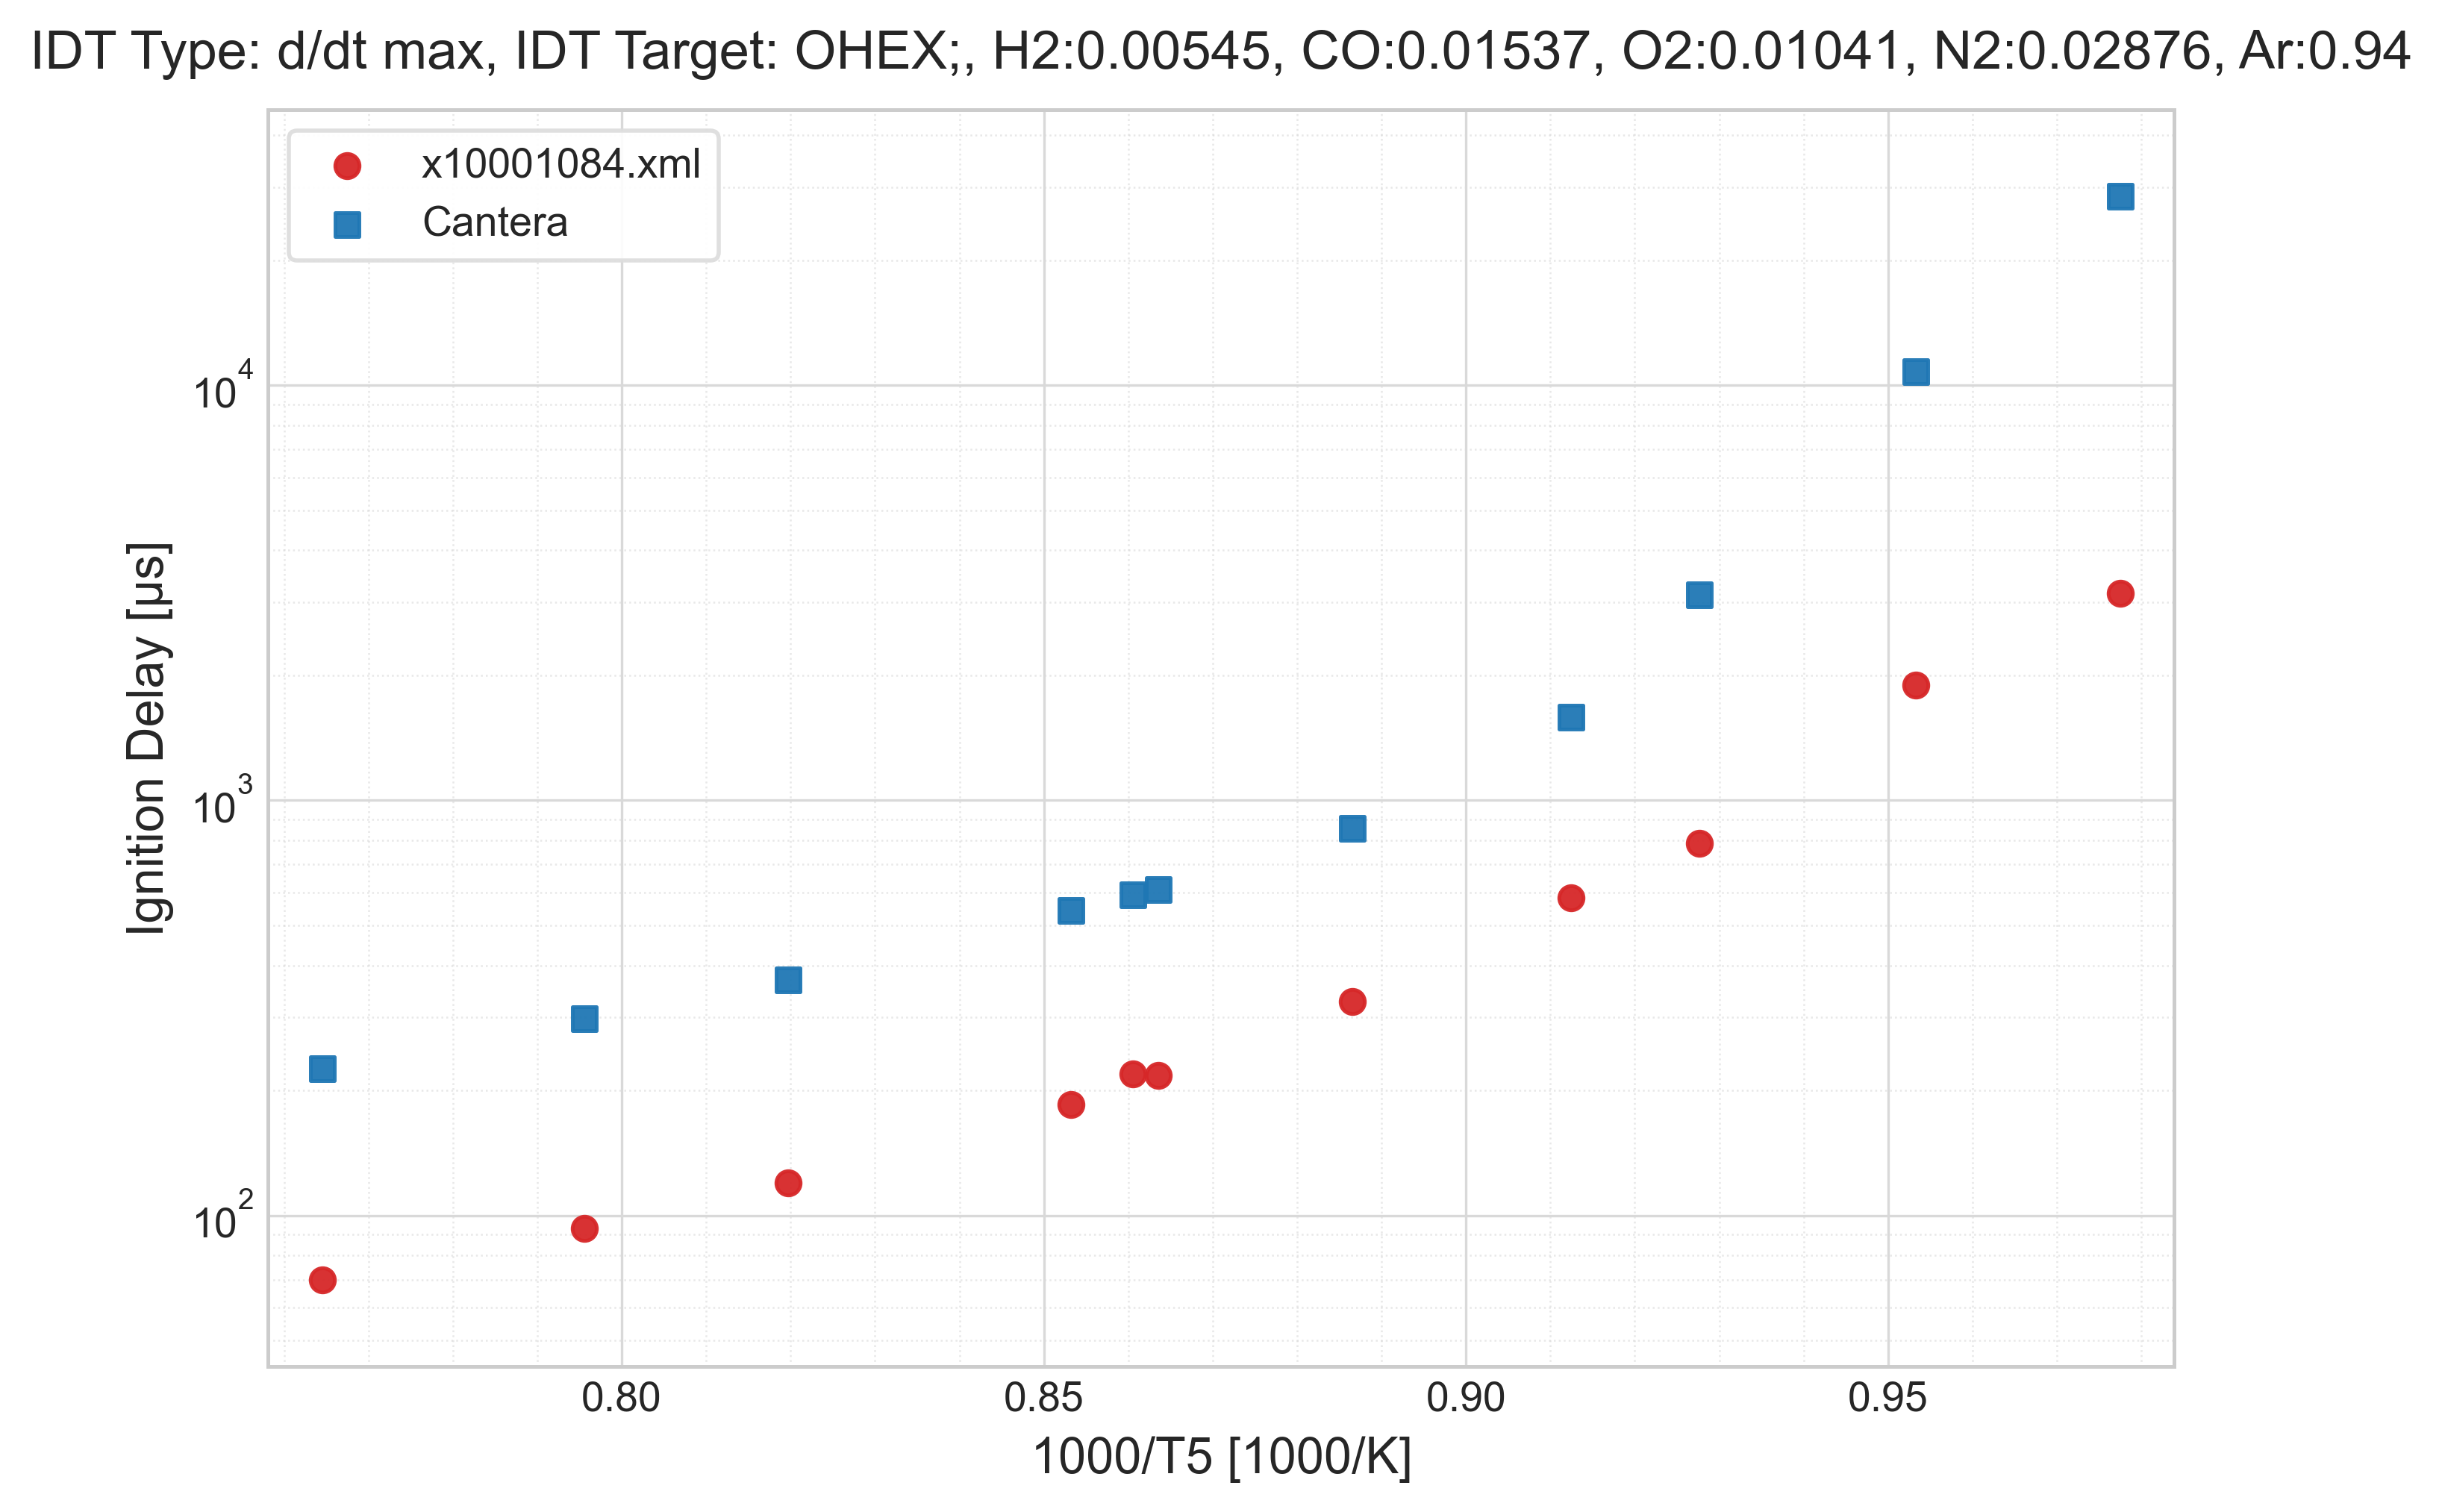
\includegraphics[width=0.8\textwidth]{Figures/IDT_plot_x10001084.png}
	\caption{Comparison of Cantera IDT simulation with experimental measurement \cite{good_cantera} IDT Type: d($OH^*$)/dt max.}
	\label{fig:bad_cantera}
\end{figure}
\begin{figure}[htbp]
	\centering
	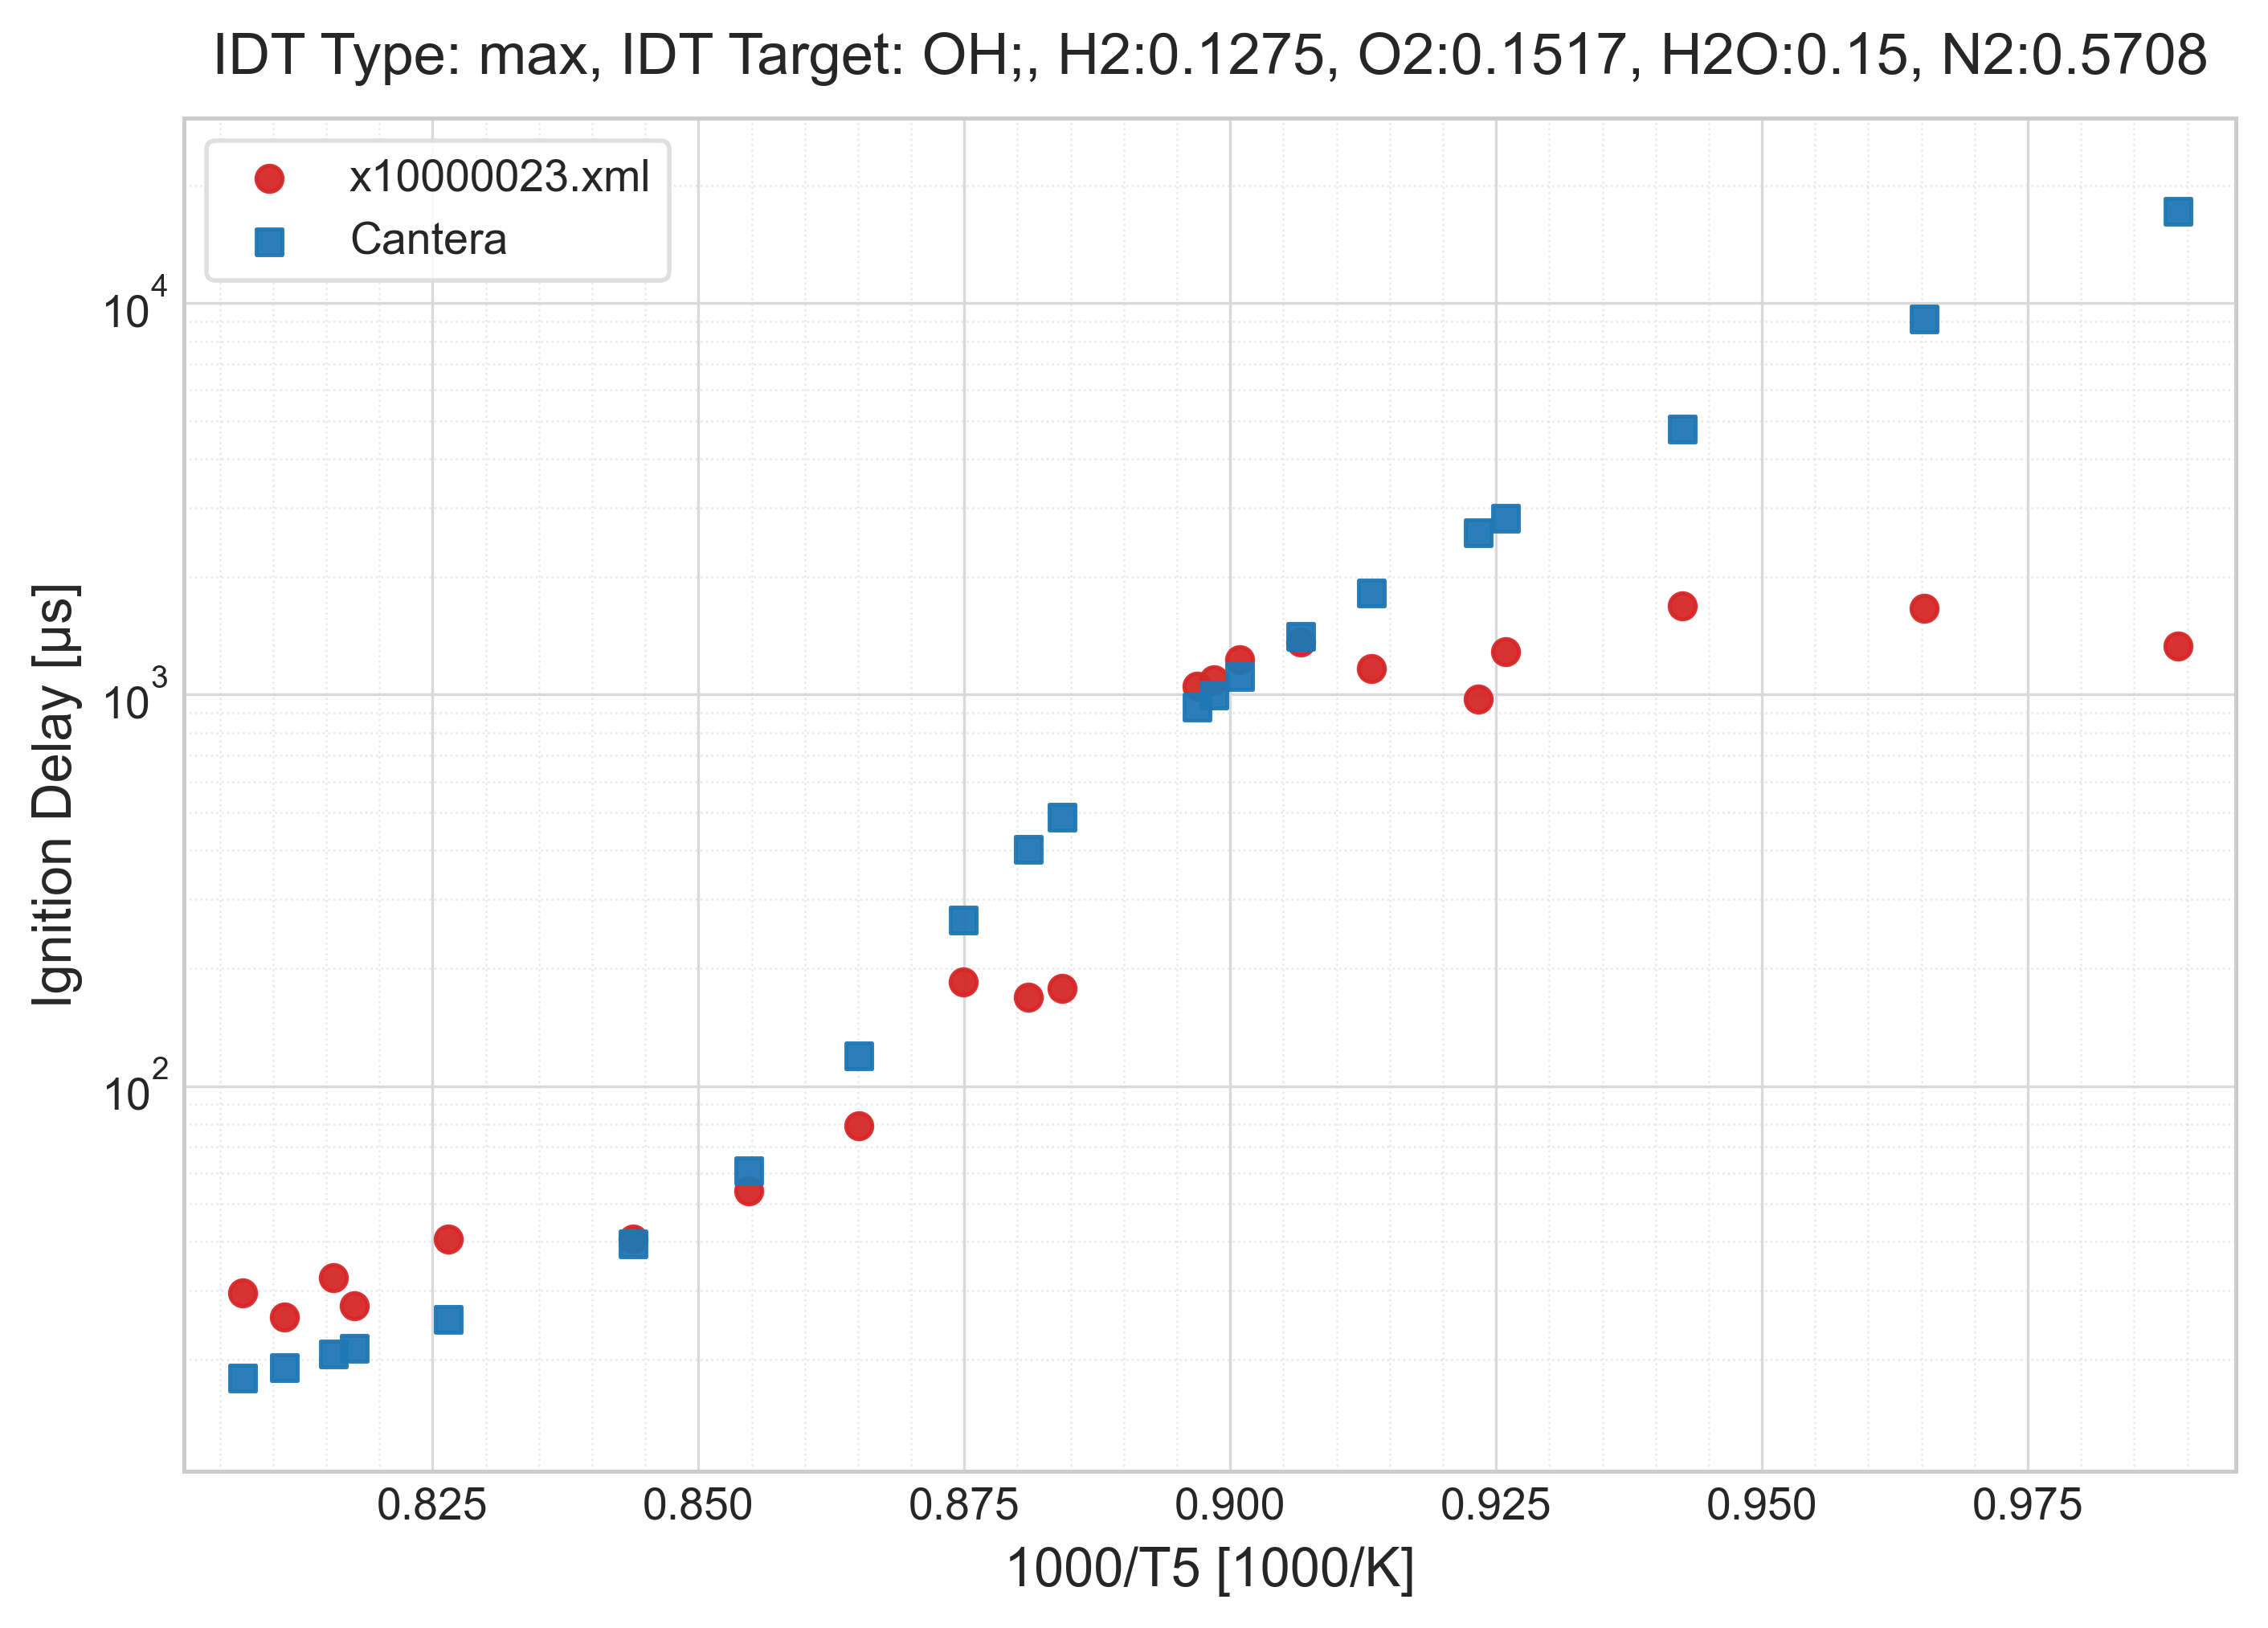
\includegraphics[width=0.8\textwidth]{Figures/IDT_plot_x10000023.png}
	\caption{Comparison of Cantera IDT simulation with experimental measurement \cite{good_cantera} IDT Type: OH max.}
	\label{fig:pressure_rise_cantera}
\end{figure}

Current implementation of Cantera IDT simulation is tested with all available Syngas and Hydrogen IDT data from RESPETCH database. \ref{fig:good_cantera}, \ref{fig:bad_cantera}, \ref{fig:pressure_rise_cantera} show some example comparisons from that dataset. 

\ref{fig:pressure_rise_cantera} illustrates the discrepency between constant volume reactor Cantera simulation and the real shock tube experiment, where boundary layer buildup reduces the effective volume. This pressure rise should be compensated for in simulation to get more accurate IDT simulations. However in the RESPETCH syngas/hydrogen IDT datasets, pressure rise is rarely reported. It would be valuable for TUMKIN database to be more comprehensive.  


\section{Consistency Analysis}

\subsection{Sensitivity Analysis}

\subsection{Surrogate Model}

\subsection{B2BDC}

\subsubsection{Reaction Mechanisms}
Reaction mechanisms used to validate the software developed in this thesis are Ethylene [18] and Combined Hydrogen Syngas [19]. Reported Chemkin input, transport and thermos files are converted to yaml by Cantera Chemkin to YAML conversion (c2kyaml).


